\chapter{RosettaHTS: A virtual High Throughput Screening tool integrating structure and ligand based information}

\section{Introduction}

\subsection{The challenge of distinguishing between active and inactive ligands by docking}

\subsection{Existing limitations in training data sources}

\subsubsection{The limitations of existing sources of active ligands}
As the goal of RosettaHTS was to train a model capable of distinguishing between active and inactive small molecules across a range of protein targets and small molecule chemical space, the selection of a high quality training set was crucial.
There are several factors which complicate the selection of a training set for a general classifier.
First, compounds with known binding affinity must be located across a wide range of protein targets.
Because the goal is to compare ligands independent of protein target, \ki\ must be used rather than \ic.
This substantially reduces the availability of data from public databased such as CHEMBL or PubChem. 
Furthermore, the active compounds selected must bind to a wide and evenly distributed range of targets, and have a wide and evenly distributed range of known activities.
Due to the realities of the drug discovery process, neither publicly nor privately available compound databases meet these requirements.
For example, while CHEMBL contains 481050 \ki\ value measurements across 164 distinct targets with known \ki values, 90\% of these targets have fewer than 891 measurements each.
In other words, nearly all of the available \ki\ values are confined to a small handful of protein targets.

\subsubsection{The limitations of existing sources of inactive ligands}
The difficulty of selecting a high quality training dataset is compounded by the availability of known inactive ligands. 
The activity data of inactive ligands is less frequently published than active ligands.
Additionally, most inactive ligands are measured as inactive by \ic\ rather than \ki.
Because \ic\ and \ki are distinct properties, a compound with no measurable \ic\ cannot necessarily be said to have no measurable binding affinity.

\subsubsection{The limitations of existing sources of active ligands}
As the goal of RosettaHTS was to train a model capable of distinguishing between active and inactive small molecules across a range of protein targets and small molecule chemical space, the selection of a high quality training set was crucial.
There are several factors which complicate the selection of a training set for a general classifier.
First, compounds with known binding affinity must be located across a wide range of protein targets.
Because the goal is to compare ligands independent of protein target, \ki\ must be used rather than \ic.
This substantially reduces the availability of data from public databased such as CHEMBL or PubChem. 
Furthermore, the active compounds selected must bind to a wide and evenly distributed range of targets, and have a wide and evenly distributed range of known activities.
Due to the realities of the drug discovery process, neither publicly nor privately available compound databases meet these requirements.
For example, while CHEMBL contains 481050 \ki\ value measurements across 164 distinct targets with known \ki values, 90\% of these targets have fewer than 891 measurements each.
In other words, nearly all of the available \ki\ values are confined to a small handful of protein targets.

\subsubsection{The limitations of existing sources of inactive ligands}
The difficulty of selecting a high quality training dataset is compounded by the availability of known inactive ligands. 
The activity data of inactive ligands is less frequently published than active ligands.
Additionally, most inactive ligands are measured as inactive by \ic\ rather than \ki.
Because \ic\ and \ki are distinct properties, a compound with no measurable \ic\ cannot necessarily be said to have no measurable binding affinity.

\subsubsection{Property matching schemes used for ligand docking benchmarks are not sufficient for training purposes}
The above-mentioned issue of the lack of known inactive compounds is frequently addressed by the use of property matching.
In this process, compounds that have similar chemical properties to the known active ligands but dissimilar structures are selected and designated as presumed inactive compounds\citep{Huang:2006gi, Mysinger:2012hu, Bauer:2013de}.
This property matching scheme can be useful for the benchmarking of ligand docking methods, but cannot be used as the basis of training data sets for machine learning techniques.
Because the property matching scheme is algorithmically selecting ligands in a slightly different part of chemical space compared to the known active ligands, the risk exists of the neural network learning to classify ligands based not on their binding affinity but rather the property matching scheme used to select them.

\subsection{ANN based methods have been effective for rescoring protein-ligand docking predictions}

\subsection{Network Dropout can be used to improve ANN generalizability}

\subsection{Network Pre-training can be used to improve ANN generalizability}

\section{Results}

\subsection{Development of a balanced training dataset}


\subsubsection{Cross-docking a diverse set of ligands to create a balanced set of training data}
\label{subsubsec:pdbbind_overview}
To address the problems above,  a cross docking approach is used to create the training dataset.
PDBBind\citep{Wang:2004cm} is a collection of Protein-ligand binding pairs for which known binding affinities and X-ray crystal structures exist.
Since it's original publication in 2004, The PDBBind database has been periodically updated, and as of 2013, contains 10776 total complexes, of which 2959 have known \ki\ values, are non-covalently bound, have only a single ligand in the binding site,  and have crystal structures with a resolution of less than 2.5 \AA.
Compounds from this "refined" subset of the PDBBind database were used as the basis of the training dataset.

\subsubsection{Additional filtering of PDBBind "refined" to produce a diverse set of high quality active compounds}
\label{subsubsec:active_poses}
For the purposes of this training set, all active ligands must have the following properties beyond those described in section \ref{subsubsec:pdbbind_overview}:
The set of proteins must be diverse, every protein in the set should come from a different family to avoid biasing training.
While RosettaLigand is capable of docking ligands into proteins into ligands of any side, extremely large proteins require the allocation of large amounts of memory, which makes screening more time consuming.
As a result, all proteins in the training set should have <1000 total residues across all chains.
RosettaLigand must be capable of predicting the pose of each complex such that the lowest Rosetta score has an RMSD of < 2.0 \AA\ to the crystal structure.
the 2959 complexes in the PDBBind refined set were filtered based on the first two criteria, and then docked using the RosettaLigand protocol described in chapter \ref{chap:lowres_paper}, resulting in a set of 507 unique protein-ligand complexes. 
This set of compounds is very diverse in chemical space, ranging from small fragments to small peptides, with the bulk of the distribution consisting of small drug-like molecules.
Specifically, the number of atoms ranges from 6 to 171, with a median of 44, the number of rings ranges from 0 to 8 with a median of 2. The number of rotatable bonds ranges from 0 to 49 with a median of 6, and the weight ranges from 87.06 to 1107.58 with a median of 107.
Figure \ref{fig:training_ligands} shows histograms of these plots.
The large diversity of this training set is desirable, as the goal is to produce a model with as wide an applicability domain as possible.

%TODO make table of all names
\begin{figure}
\centering
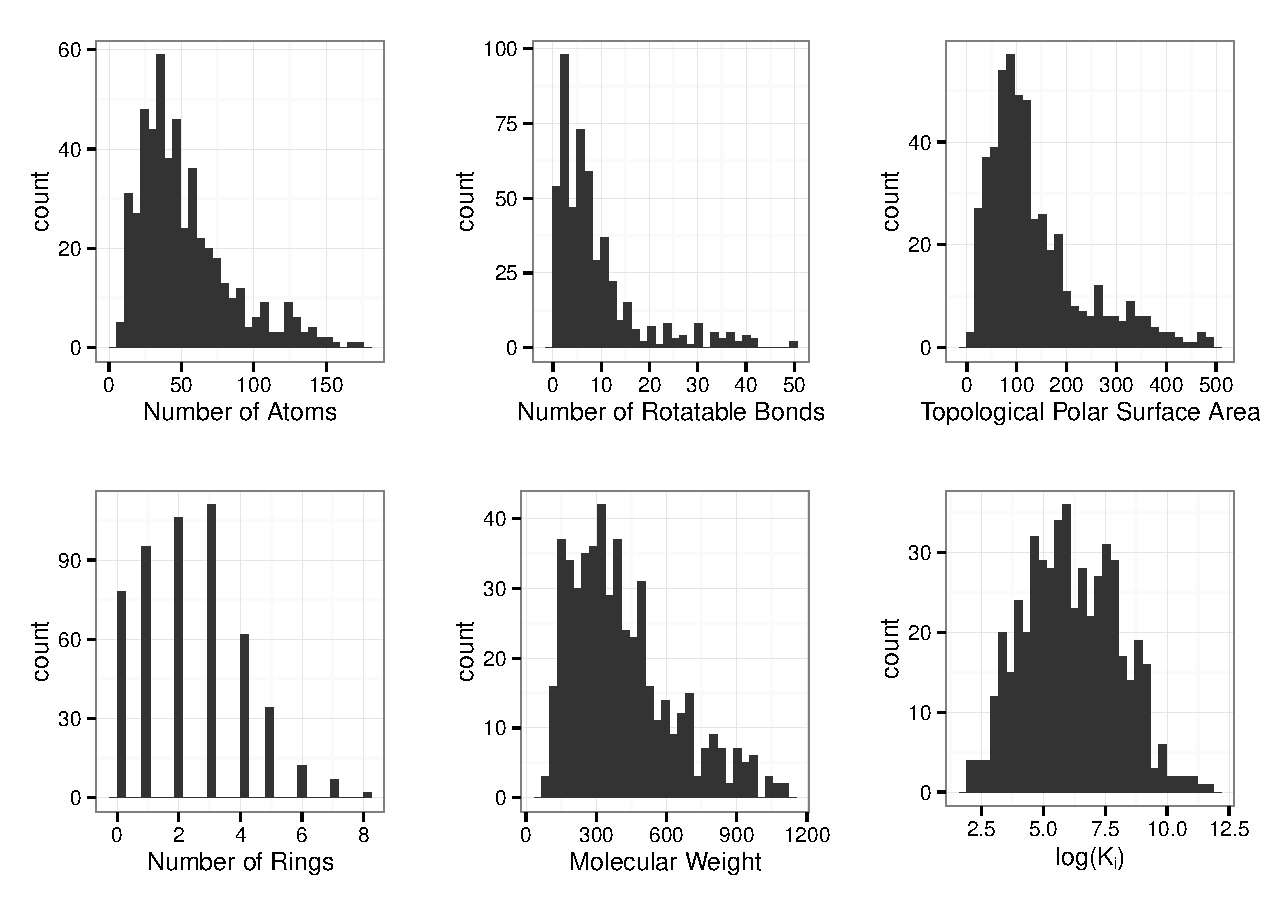
\includegraphics[width=4in]{figures/hts/basic_ligand_properties.pdf}
\caption{
The basic property distribution of ligands in the training data set.  Histograms are plotted of the atom count, rotatable bond count, ring count, Topological Polar Surface area, log(\ki) and molecular weight of the 507 ligands in the binding site. 
}
\label{fig:training_ligands}
\end{figure}

\subsubsection{Crossdocking active compounds produces presumed inactive binding data}
The best scoring, lowest RMSD binding poses selected in section \ref{subsubsec:active_poses} will comprise the active component of the training set.
The inactive component of the training set was generated through cross-docking.
Each ligand in the 507 compound set was docked into each of the proteins in the set except the one with measured activity data.
Due to the size of chemical space\citep{Reymond:2012un} and the diversity of the protein-ligand complexes in the dataset, it can be reasonably assumed that every cross-docked complex has no binding affinity.
The lowest scoring Rosetta model for each cross-docked complex was selected, and the resultant set of 250970 protein-ligand complexes will comprise the inactive component of the training set.

\subsection{Development and description of ligand descriptors}

\subsubsection{Sources of descriptor data} 

The proper selection of descriptors is critical for the training of an effective model.
It is frequently difficult to determine \textit{a priori} which descriptors will be the most useful, so three classes of descriptor information were evaluated.  Specifically: scalar scores and statistics describing the protein-ligand interface,  RDF descriptors describing the arrangement of atoms in the protein-ligand interface, and scalar metrics describing the ligand chemistry.

\subsubsection{Scalar protein-ligand interface descriptors}
\label{subsubsec:scalar_rosetta}
The RosettaLigand energy function directly provides a number of metrics that can be used as scalar descriptors of the chemistry of the protein-ligand interface.
In addition to these scores, Rosetta implements an "Interface Analyzer" which generates additional descriptors of the protein-ligand interface.
Between these two descriptor sources, a set of 20 descriptors can be computed, describing the van der waals, hydrogen bonding, desolvation and electrostatic energy of the protein-ligand interface, as well as the size of the protein binding pocket, the number of unsatisfied hydrogen bonds, and the Solvent Accessible Surface Area(SASA) of the interface.
Table \ref{table:rosetta_scalar} summarizes the specific scalar interface descriptors used.
\begin{table}
\scriptsize
\renewcommand{\tabcolsep}{0.09cm}
\centering
\begin{tabular}{|c|c|}
\hline
Property name & Description \\
\hline
\multicolumn{2}{|c|}{\textbf{Rosetta energy descriptors}} \\
\hline
if\_X\_fa\_atr & Attractive force of the protein-ligand interface\\
\hline
if\_X\_fa\_rep & Repulsive force of the protein-ligand interface\\
\hline
if\_X\_fa\_intra\_rep & Repulsive force between atoms in each residue and the ligand \\
\hline
if\_X\_fa\_elec & Electrostatic force of the protein-ligand interface \\
\hline
if\_X\_fa\_pair & The value of the Rosetta pair energy between protein and ligand residues\\
\hline
if\_X\_fa\_sol & The desolvation energy of the protein-ligand interface \\
\hline
if\_X\_hbond\_bb\_sc & The hydrogen bonding energy between protein backbone atoms and ligand atoms \\
\hline
if\_X\_hbond\_sc & The hydrogen bonding energy between protein side chain atoms and ligand atoms \\
\hline
hbond\_lr\_bb & The long range hydrogen bonding energy between protein backbone atoms in the entire complex \\
\hline
hbond\_sc & The hydrogen bonding energy between all side chain atoms in the entire complex\\
\hline
hbond\_sr\_bb &  The long range hydrogen bonding energy between protein backbone atoms in the entire complex\\
\hline
interface\_delta\_X & The total Rosetta score associated with the protein-ligand interface\\
\hline
total\_score/nres\_all & The total complex score divided by the total number of protein residues \\
\hline
\multicolumn{2}{|c|}{\textbf{Rosetta Interface Analyzer descriptors}} \\
\hline
dSASA\_hydrophobic & The hydrophobic SASA at the protein-ligand interface  \\
\hline
dSASA\_int & The total SASA at the protein-ligand interface  \\
\hline
dSASA\_polar & The polar SASA at the protein-ligand interface \\
\hline
delta\_unsatHbonds & The number of unsaturated hydrogen bonds at the protein-ligand interface\\
\hline
hbond\_E\_fraction & The fraction of the interface energy associated with hydrogen bonding\\
\hline
nres\_int & The number of protein residues at the protein-ligand interfaec\\
\hline
packstat & The protein-ligand interface packing statistic originally described by Sheffler \citep{Sheffler:2009bd} \\
\hline
\end{tabular}
\caption{A summary of the names and definitions of the scalar descriptors generated by Rosetta.
Rosetta energy descriptors were originally described by Rohl\citep{Rohl:2004dh} }
\label{table:rosetta_scalar}
\end{table}

\subsubsection{Scalar ligand descriptors}

The scalar descriptors discussed in section \ref{subsubsec:scalar_rosetta} encode only information related to the protein-ligand interface. 

\section{Discussion}



\section{Methods}